\problemname{Röð}

Hópur af $n$ krökkum ætlar að fara að spila Asna, fótboltaleikur sem skiptir
ekki máli í þessu verkefni. Til þess þurfa þau að mynda röð, en þau eiga erfitt
með að ákveða röðina. Sem betur fer er hún Gunna litla klár, og kann aðferð til
að ákveða röðina á slembinn hátt.

Krakkarnir eru fyrst númeraðir með bókstöfum $A, B, C, \ldots$. Svo eru sömu
bókstafir skrifaðir niður á blað, og tölurnar $1,\ldots,n$ skrifaðir niður á
móti þeim. Lóðréttar línur eru svo teiknaðar á milli samsvarandi bókstafs og
tölu. Ef við gerum ráð fyrir að það séu $6$ krakkar, þá lítur blaðið núna út
eins og á eftirfarandi mynd:

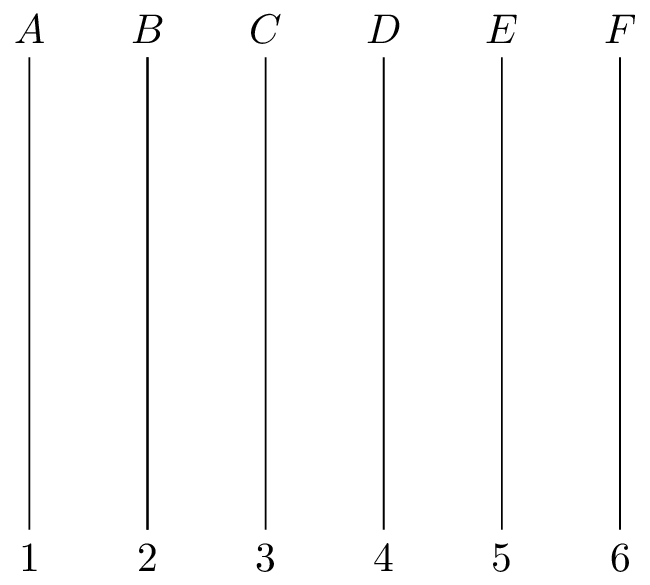
\includegraphics[width=0.6\textwidth]{empty.png}

Núna eru láréttar línur teiknaðar á milli samliggjandi lóðréttra lína á
handhófskenndum stöðum. Láréttu línurnar mega þó aldrei snertast. Nú gæti
blaðið litið út eins og á eftirfarandi mynd:

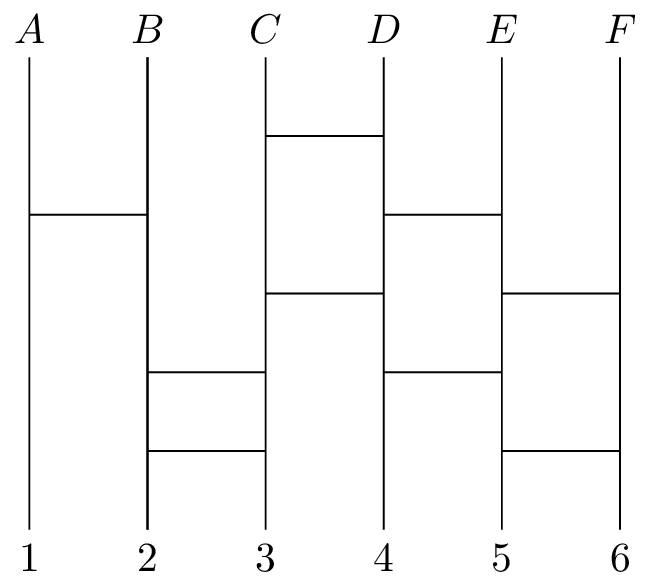
\includegraphics[width=0.6\textwidth]{with_lines.png}

Til að ákvarða hvar ákveðinn krakki er í röðinni, þá byrjar maður hjá
bókstafnum sem krakkinn hefur, og fylgir svo lóðréttu línunni niður. Þegar
maður kemur að láréttri línu sem snertir línuna sem maður er á, þá fylgir maður
láréttu línunni yfir að næstu lóðréttu línu og heldur áfram niður. Þetta gerir
maður þangað til maður kemur að tölustaf. Þessi tölustafur táknar hvar krakkinn
er í röðinni. Eins og eftirfarandi mynd sýnir, þá yrði krakkinn með bókstaf $E$
númer $3$ í röðinni.

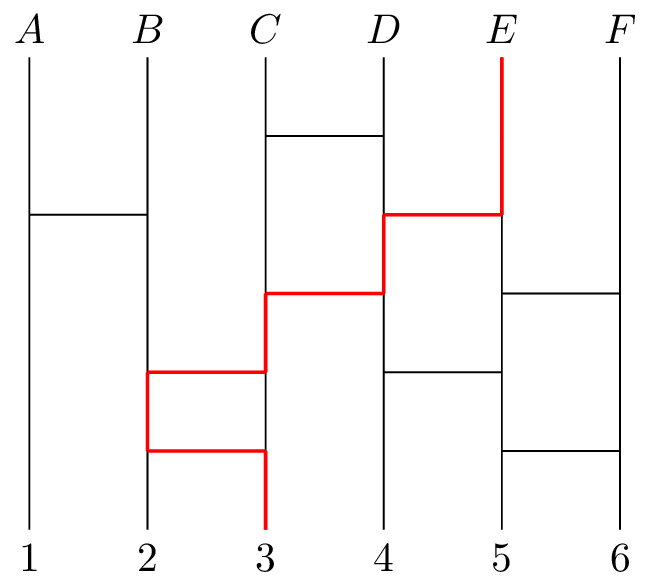
\includegraphics[width=0.6\textwidth]{path.png}

Á fyrstu línu inntaksins eru heiltölurnar $1 \leq n \leq 26$ og $1 \leq k \leq
100$, aðskildar með bili. Þar á eftir fylgja $k$ línur sem tákna blaðið sem
krakkarnir teiknuðu.

Úttak á að innihalda eina línu með $n$ bókstöfum, sem er röðin sem krakkarnir
mynda eftir að þeir hafa notað blaðið. Fremsti bókstafurinn táknar þann sem er
fyrstur í röðinni.

